\documentclass[12pt]{article}


\author{Fl\'{a}vio Cruz and Richard Veras}
\title{Assignment 1}

\usepackage{amsmath}
\usepackage{amsfonts}   % if you want the fonts
\usepackage{amssymb}    % if you want extra symbols
%\usepackage{savetrees}
\usepackage{algorithmic}
\usepackage{graphicx}
\usepackage{listings}


\begin{document}
\maketitle

\section{Pass 1 - Meet the functions}

For this pass, we implemented a data structure, \texttt{info}, that contains all the statistics of a function. We also have a dictionary (implemented as a \texttt{map})
   that maps function names to \texttt{info}. For each function, we collect all the basic information that is available through the \texttt{Function} class. To count the number
   of blocks and instructions, we use the blocks iterator and sum the number of instructions per block. Finally, to count the number of call sites, we iterate over the code of
   the module (by blocks) and check for \texttt{CallInst} instructions.

\section{Pass 2 - Optimize the Block}

This pass iterates over all the blocks of the module and performs two operations:

\begin{itemize}
   \item Simple Optimizations: algebraic identities, strengh reductions, and identities.
   \item Constant Folding: constants are folded and certain instructions (like dead \texttt{store}'s).
   \item Removal of \texttt{alloca} instructions: certain instructions that are no longer used inside the block.
\end{itemize}

\subsection{Simple Optimizations}

In this phase, we iterate over the instructions of a block. We use a stack of \texttt{load} instructions, where we push (at most) the latest two \texttt{load} instructions.

When the stack contains 2 \texttt{load}'s, it means that both places are actually the same (we check this). This fact is used to optimize divisions (x/x) when a division operation
appears next. Here, we delete both \texttt{load}'s and replace the division instruction with a constant value (using \texttt{ReplaceInstWithValue}).


When the stack contains only 1 \texttt{load}, we may perform the other algebraic identities ($x + 0$, $x / 1$, $x * 2$, $x / 2$, etc). We check if one operand is a constant value and perform
the corresponding replaces and deletion of the load instruction. We also perform a simple optimization when we have a \texttt{load} followed by a \texttt{store} to the same place,
    by deleting both instructions. This last situation may happen because of other optimizations.

\subsection{Constant Folding}

In constant folding, we also iterate over the instructions of a basic block. We maintain a dictionary (\texttt{map}), that maps \texttt{Value}'s to \texttt{Value}'s, where the latter is a constant value.

Whenever we have a store where the content is a constant, we add this fact to the dictionary (by taking the store destination and value) and we also remove the store since it's not needed anymore. (Note however, that we don't remove the last store that is used for function return). Next, when we find some \texttt{load} instruction that attempts to load some value that is present in our dictionary, we use
\texttt{ReplaceInstWithValue}, which automatically removes this \texttt{load} instruction and every reference to this value (before the next store).

The most interesting part is when operations, due to so many replaces, are applied to constant arguments. Here, we read both constants and compute the final value and then we replace the instruction with the computed value, again with \texttt{ReplaceInstWithValue}.

\subsection{Removal of \texttt{alloca}}

In this final phase, we remove certain instructions that are dead. For this we check if the instruction (the value) isn't used anywhere, by executing \texttt{use\_empty}.

\section{Code - Meet the Functions}

{\tiny \lstinputlisting{../FunctionInfo/FunctionInfo.cpp}}

\section{Code - Optimize the Block}

{\tiny \lstinputlisting{../LocalOpts/LocalOpts.cpp}}

\section{Tests Cases for Meet the Functions}

\subsection{Loop}

{\tiny \lstinputlisting{../FunctionInfo/loop.c}}

\subsection{Other}

{\tiny \lstinputlisting{../FunctionInfo/other.c}}

\section{Tests Cases for Optimize the Block}

\subsection{Strength}

{\tiny \lstinputlisting{../LocalOpts/strength.c}}

\subsection{Constfold}

{\tiny \lstinputlisting{../LocalOpts/constfold.c}}

\subsection{Algebraic}

{\tiny \lstinputlisting{../LocalOpts/algebraic_orig.c}}

\subsection{Other}

{\tiny \lstinputlisting{../LocalOpts/algebraic.c}}




\section{Problems}

\subsection{CFG Basics}

%\begin{figure}[h]
\begin{minipage}[b]{0.5\linewidth}
\centering


\begin{tabular}{| l l| l}
%  LABEL& EXPR & BASIC BLOCK \\
  \cline{0-1}
  & $x = 100$ & BB0 \\
  & $y = 0$ &  \\
  & goto L2 &  \\
  \cline{0-1}
  L1: & $y = x * y$ & BB1 \\
  & $ \operatorname{if}(x < 50 )$ goto L2 &  \\
  \cline{0-1}
  & $y = x - y$ &  BB2\\
  & goto L3 & \\
  \cline{0-1}
  L2: & $y = x + y$ & BB3 \\
  \cline{0-1}
  L3: & $\operatorname{print}(y)$ & BB4 \\
  & $ \operatorname{if}(y < 1000 )$ goto L1 &  \\
  \cline{0-1}
  & $ \operatorname{if}(x \le 0 )$ goto L5 & BB5  \\
  \cline{0-1}
  L4: & $x = x-1$ & BB6 \\
  & goto L1 & \\
  \cline{0-1}
  L5: & return y & BB7 \\
  \cline{0-1}

\end{tabular}

%\caption{ Here we have the basic blocks of this code sample labeled. }
\label{fig:figure1}
\end{minipage}
\hspace{0.5cm}
\begin{minipage}[b]{0.5\linewidth}
\centering


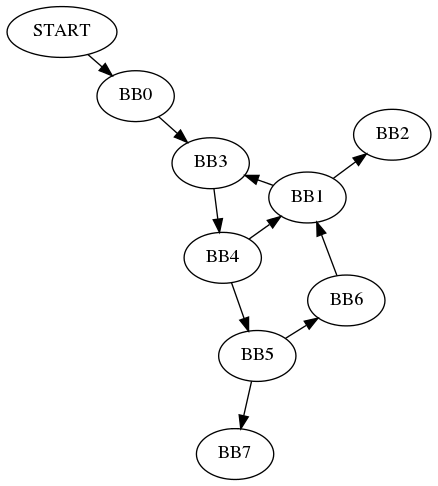
\includegraphics[scale=.3]{prob_51_cfg.png}


%\caption{This graph corresponds to the control flow graph of our code sample.}
\label{fig:figure2}
\end{minipage}
%\end{figure}







\subsection{Available Expressions}

\begin{enumerate}
\item
\begin{tabular}{| l| l| l|}
  \hline
  BB & EVAL & KILL \\
  \hline
  1 & $ { d_1, d_2, d_3, d_4}$ & ${ d_5, d_6, d_7, d_8, d_9, d_{10}, d_{11},
      d_{12}} $ \\
  2 & ${ d_5, d_6, d_7 }$ & ${d_9}$ \\
  3 & ${d_8, d_9}$ & ${d_6, d_{12}}$  \\
  4 & ${d_{10}, d_{11}}$  & ${d_8}$  \\
  5 & ${d_{12}}$  & ${d_4}$  \\
  \hline
\end{tabular}

\item
\begin{tabular}{| l| l| l|}
  \hline
  BB & IN & OUT \\
  \hline
  1 & $\emptyset$ & ${ d_1, d_2, d_3, d_4}$ \\
  2 & ${ d_1, d_2, d_3, d_4, d_5, d_6, d_7, d_8, d_9, d_{10}, d_{11}, d_{12}}$
  & ${ d_1, d_2, d_3, d_4, d_5, d_6, d_7, d_8, d_{10}, d_{11}, d_{12}}$ \\
  3 & ${ d_1, d_2, d_3, d_4, d_5, d_6, d_7, d_8,d_{10}, d_{11}, d_{12}}$ & ${
    d_1, d_2, d_3, d_4, d_5, d_7, d_8, d_9, d_{10}, d_{11}}$ \\
  4 & ${ d_1, d_2, d_3, d_4, d_5, d_6, d_7, d_8, d_{10}, d_{11}, d_{12}}$ & ${ d_1, d_2, d_3, d_4, d_5, d_6, d_7, d_9, d_{10}, d_{11}, d_{12}}$ \\
  5 & ${ d_1, d_2, d_3, d_4, d_5, d_6, d_7, d_8, d_9, d_{10}, d_{11}}$ & ${ d_1, d_2, d_3,  d_5, d_6, d_7, d_8, d_9, d_{10}, d_{11}, d_{12}}$ \\
  \hline
\end{tabular}
\end{enumerate}

\subsection{use-without-def}
\begin{enumerate}

\item The elements we are operating on in our analysis is the set of
  definitions, both real definitions and dummy definitions.

\item In this analysis we move from top to bottom, just like in the analysis
  for reaching definitions.

\item Our transfer functions are identical to those in the reaching definition
  analysis. Namely:

  \begin{equation}
    f_b(x) = \operatorname{GEN}_b \cup (\operatorname{IN}[b] - \operatorname{KILL}_b)
  \end{equation}

Where, $\operatorname{GEN}_b$: is the set of definitions exposed in the basic
block $b$. $\operatorname{IN}[b] = \bigcup_{P\in pred\, block}OUT[P]$ and $\operatorname{KILL}_b$ is the
definitions in basic block $b$ that are killed.

\item Our meet operation is set union, $\cup$.

\item We initialize the Exit and Entry nodes as follows:

  \begin{equation}
    \operatorname{OUT}[\operatorname{ENTRY}] = {d^{dummy}_i| i \in
      \operatorname{vars}}
  \end{equation}

  \begin{equation}
    d^{dummy}_i: i := \operatorname{dummy-value}
  \end{equation}

Where $\operatorname{vars}$ is the set of all variables in our program.

\item All of the $IN$ and $OUT$ sets are initialized to $\emptyset$.

\item The ordering does not affect correctness, but because we are chasing
  these dummy definitions down the control flow graph it would be useful to
  use a depth-first traversal.

\item Our analysis will converge because we are dealing with a monotone meet
  function and a finitely sized set.

\item

\begin{algorithmic}
$\operatorname{OUT}[\operatorname{ENTRY}] = {d^{dummy}_i| i \in
      \operatorname{vars}}$
\FORALL {Basic Blocks B other than ENTRY }
    \STATE $\operatorname{OUT}[B]=\emptyset$
\ENDFOR

\WHILE {Changes occur to any other OUT}
    \FORALL  {Basic Blocks B other than ENTRY }
        \STATE $\operatorname{IN}[B] = \bigcup_{P\in pred\, block}OUT[P]$
        \IF {$\operatorname{IN}[B]$ does not contain a dummy variable}
            \STATE \emph{Break}
        \ENDIF

        \STATE $\operatorname{OUT}[B]= \operatorname{GEN}_B \cup (\operatorname{IN}[B] - \operatorname{KILL}_B)$
        \IF {$\operatorname{GEN}_B$  used a dummy variable}
            \STATE Flag use-without-def
        \ENDIF
    \ENDFOR
\ENDWHILE


\end{algorithmic}


\end{enumerate}



\end{document}
